\documentclass[11pt]{article}
\usepackage[a4paper,hscale=0.74,vscale=0.95]{geometry}

%\usepackage[latin1]{inputenc}
%\usepackage{charter}
\usepackage[german,english]{babel}
%\usepackage{url}
%\usepackage{pdfsetup}
\usepackage{eurosym}
\usepackage{graphicx}
\usepackage{verbatim}
%\usepackage{float}
\usepackage{tikz}

\usepackage[justification=centering]{caption}

\usepackage{xeCJK}
\setCJKmainfont[BoldFont=STZhongsong, ItalicFont=STKaiti]{STSong}
\setCJKsansfont[BoldFont=STHeiti]{STXihei}
\setCJKmonofont{STFangsong}

\parindent 0pt
\parskip 1ex
\begin{document}
\setcounter{tocdepth}{1}

\newcommand{\alert}[1]{{\color{red}{#1}}}

\begin{center}
{\Large\bf A Detailed Travel Guide \\
	 from Nanjing Lukou Airport to Hanyuan Hotel}
\end{center}

Nanjing Lukou International Airport (南京禄口国际机场, IATA: NKG) has direct flight
from Frankfort every Wednesday, as well as many domestic flights.
NKG has two terminals (T1 and T2), and only T2 is currently used.
Fig.~\ref{drawing} is a simplified map of T2.
\begin{figure}[!h]
    \centering
    	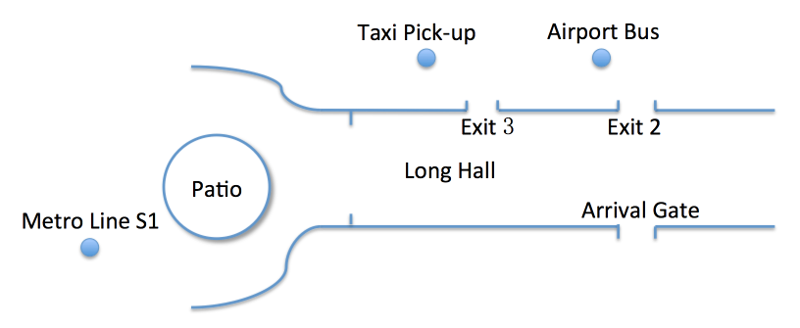
\includegraphics[scale=0.9]{jjj.png}
    	\caption{Map of T2.\label{drawing}}
 \end{figure}

There are three options to go from NKG to Hanyuan hotel as listed below.

\begin{center}
 \begin{tabular}{| c | p{3.5cm} | p{3cm} | p{3.5cm}| }
  	\hline
	\textbf{Option} 	&	\bf{Via}					& \bf{Cost	}			& \bf{Time} 				 \\
	\hline
	1						&	Metro + Taxi			& \textyen 6 +  \textyen 25		& 35 + 20 minutes 	\\
	\hline
	2						&	Taxi				 		& \textyen 130 			& 45 minutes \\
	\hline
	3						& Airport Bus + Taxi	& \textyen 20 + \textyen 25 		& 45 + 20 minutes \\			 
	\hline
\end{tabular}
\end{center}

\section{Metro + Taxi}

This one is the recommended, which consists of two hops:

 \begin{center}
 \begin{tabular}{| l | p{4.5cm} | p{4.5cm} | p{2.5cm}|}
  	\hline
	\textbf{Hop} 	&	\bf{From}		& \bf{To	}														 & \bf{By} \\
	\hline
	1					&	NKG				& Nanjing South Railway Station(南京南站)	& Metro Line S1\\
	\hline
	2					&	Nanjing South Railway Station (南京南站)%		
												& Hanyuan Hotel (翰苑)			    & Taxi	\\
	\hline
\end{tabular}
\end{center}

\subsection{Details of Hop 1}

S1 starts at 6:40 am and ends at 22:00 pm.
The following figures show how to get to S1 by following overhead directions.
\begin{figure}[!h]
    \centering
    	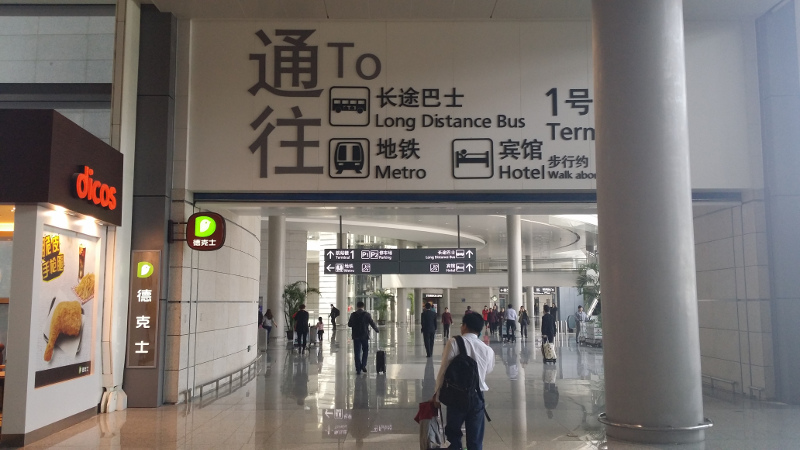
\includegraphics[scale=0.27]{20150331_105936.jpg}
    	\caption{Walk along the long hall, you will see a big sign above the door in front of you.\label{20150331_105936}}
 \end{figure}
\begin{figure}[!h]
    \centering
    	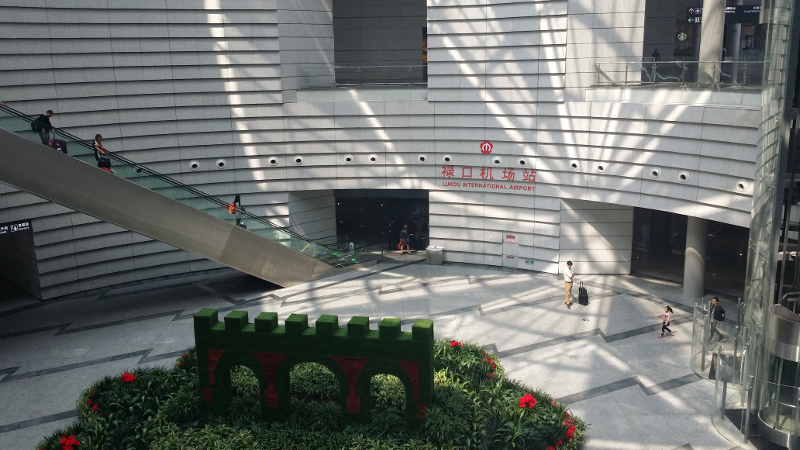
\includegraphics[scale=0.27]{20150331_110112.jpg}
    	\caption{Keep walking you will see an escalator on your left.\label{20150331_110112}}
 \end{figure}
 \begin{figure}[!h]
    \centering
    	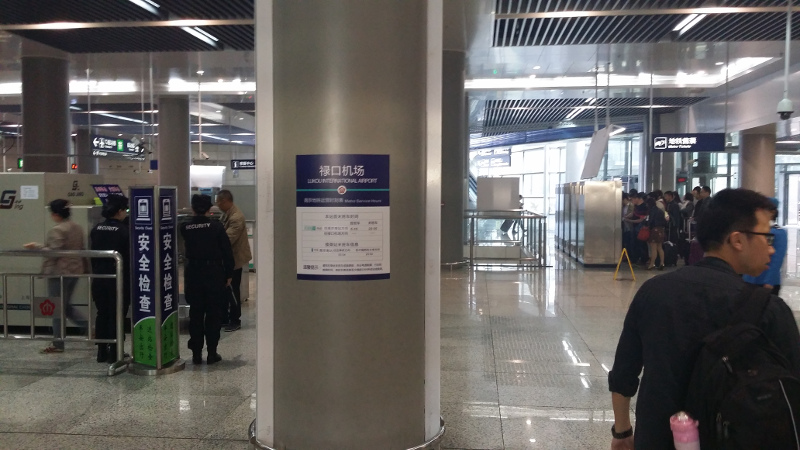
\includegraphics[scale=0.27]{20150331_110303.jpg}
    	\caption{Take the escalator downstairs, you will see the security check on your left and ticket machines on your right.\label{20150331_110303}}
 \end{figure}
\begin{figure}[!h]
	\begin{minipage}[t]{.5\textwidth}
     	\centering
        	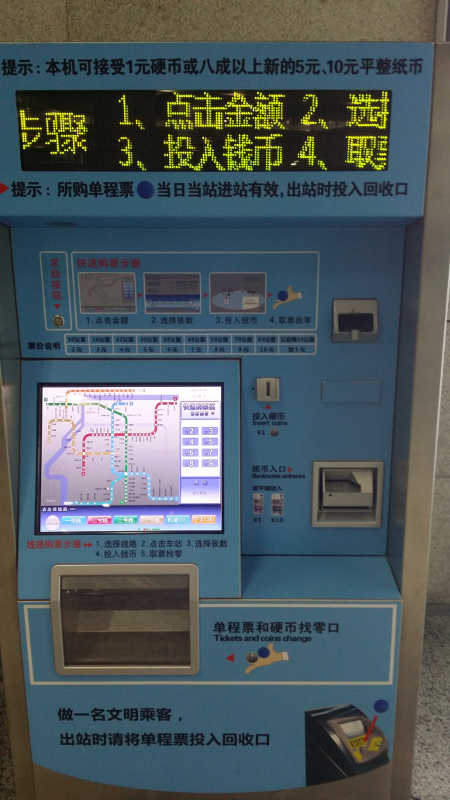
\includegraphics[scale=0.27]{20150331_110412.jpg} \\
		\caption{A Metro ticket machine.\label{20150331_110412}}
	\end{minipage}%
     \begin{minipage}[t]{.5\textwidth}
         \centering
       	 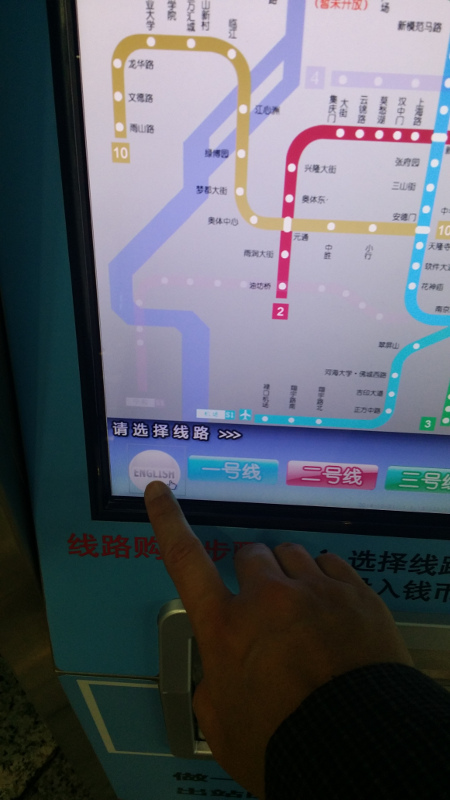
\includegraphics[scale=0.27]{20150331_110433.jpg} \\
	 	\caption{Change the language to English .\label{20150331_110412}}
    \end{minipage}%
 \end{figure}
 \begin{figure}[!h]
	\begin{minipage}[t]{.5\textwidth}
     	\centering
        	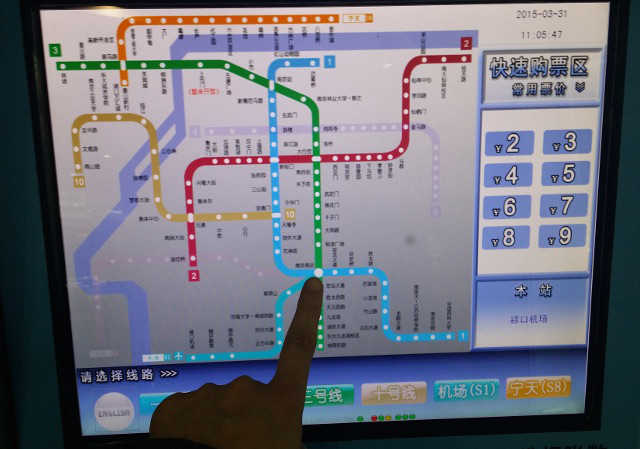
\includegraphics[scale=0.27]{20150331_110548.jpg}
		\caption{Press screen here.\label{20150331_110548}}
	\end{minipage}%
     \begin{minipage}[t]{.5\textwidth}
         \centering
       	 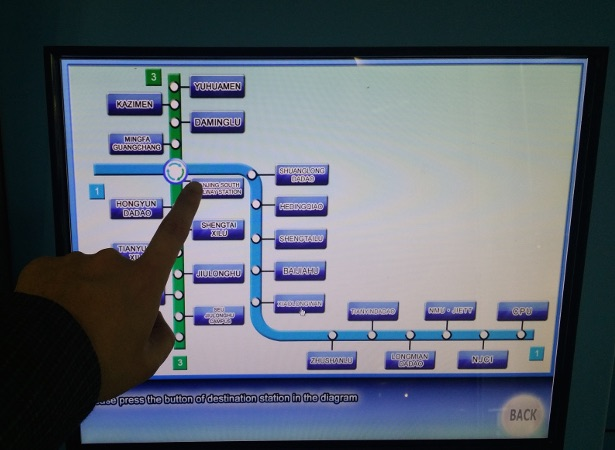
\includegraphics[scale=0.27]{20150331_110629.jpg}
	 	 \caption{Press screen here.\label{20150331_110629}}
    \end{minipage}%
 \end{figure}
 \begin{figure}[!h]
	\begin{minipage}[t]{.5\textwidth}
     	\centering
        	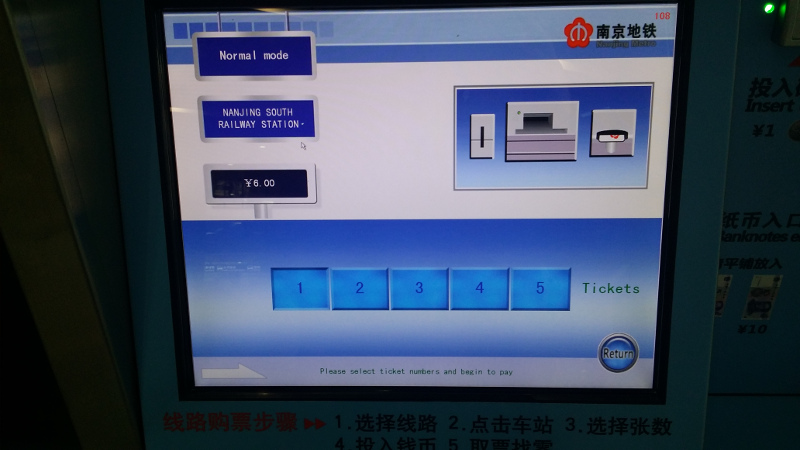
\includegraphics[scale=0.27]{20150331_110642.jpg}
		\caption{\textyen 6 for 1 ticket.\label{20150331_110642}}
	\end{minipage}%
     \begin{minipage}[t]{.5\textwidth}
         \centering
       	 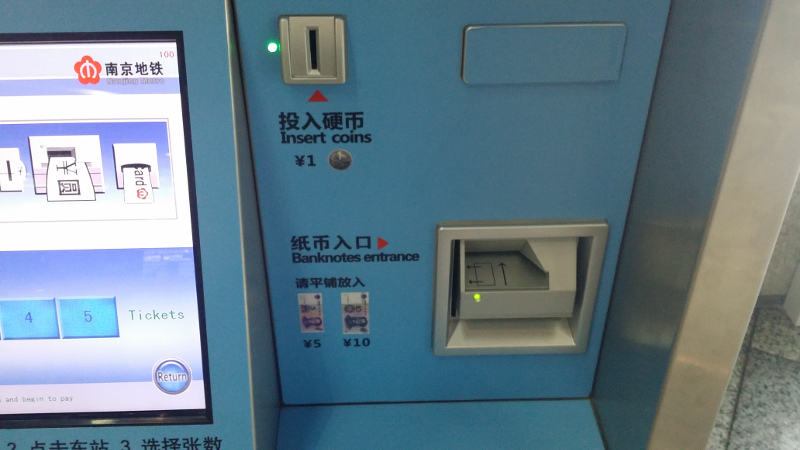
\includegraphics[scale=0.27]{20150331_110651.jpg}
	 	 \caption{Only \textyen 5 bills,  \textyen10 bills and \textyen 1 coins are acceptable. 
		 	You can always change large bills at the service spots inside Metro station.\label{20150331_110651}}
    \end{minipage}%
 \end{figure}
  \begin{figure}[!h]
	\begin{minipage}[t]{.5\textwidth}
     	\centering
        	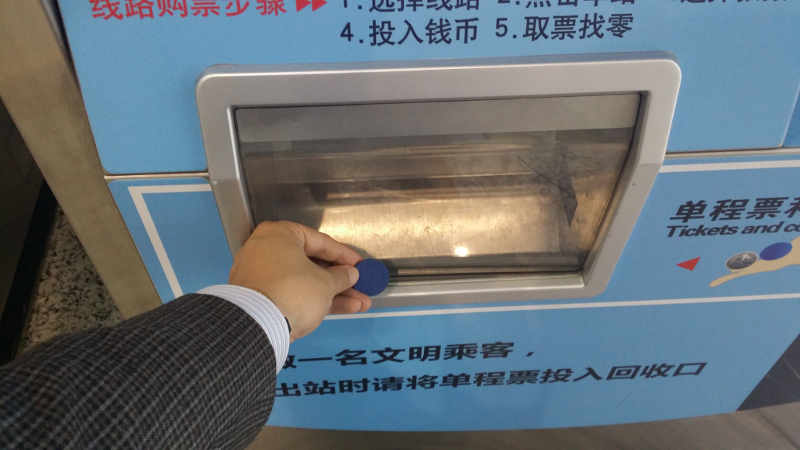
\includegraphics[scale=0.27]{20150331_110738.jpg}
		\caption{The plastic blue coin is your ticket. \label{20150331_110738}}
	\end{minipage}%
     \begin{minipage}[t]{.5\textwidth}
         \centering
       	 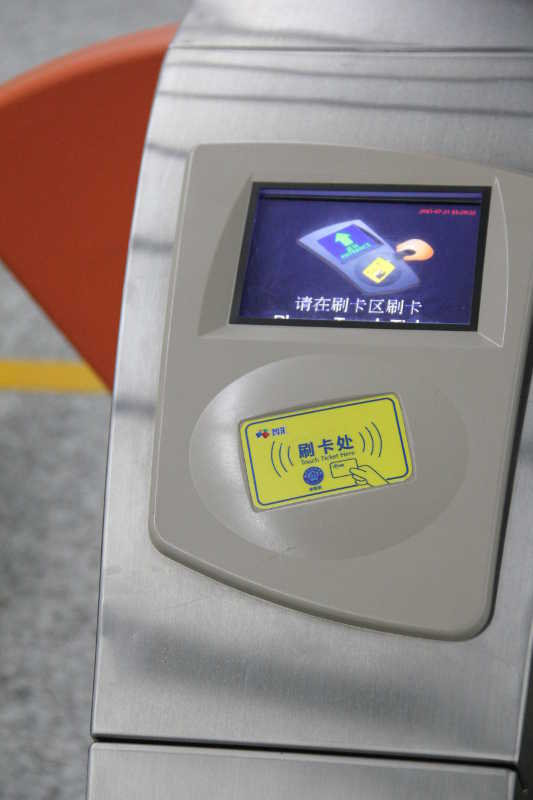
\includegraphics[scale=0.27]{IMG_7177.jpg}
	 	 \caption{Swipe the ticket over this area. \label{IMG_7177}}
    \end{minipage}%
 \end{figure}
 \begin{figure}[!h]
	\begin{minipage}[t]{.5\textwidth}
     	\centering
        	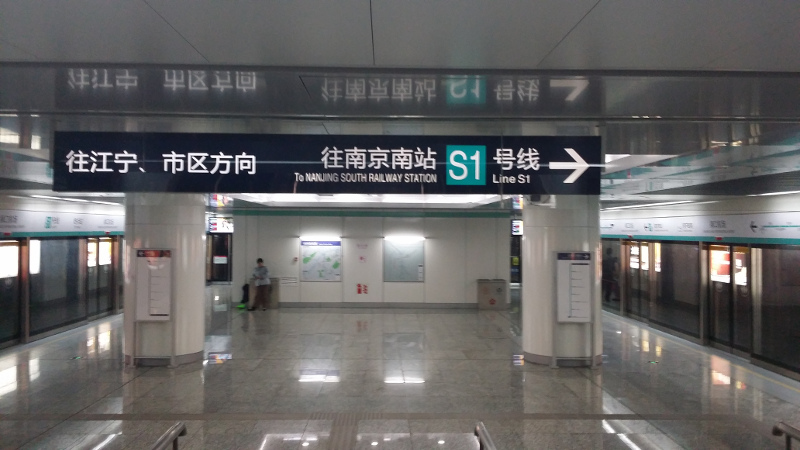
\includegraphics[scale=0.27]{20150331_110903.jpg}
    		\caption{Take the escalator downstairs, \protect \\ and the train is on the right side. \label{20150331_110903}}
	\end{minipage}%
     \begin{minipage}[t]{.5\textwidth}
         \centering
       	 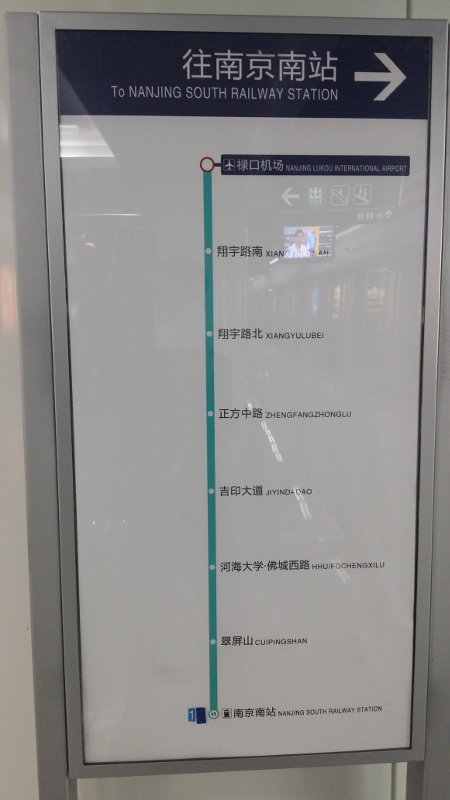
\includegraphics[scale=0.27]{20150331_110935.jpg}
		\caption{Nanjing South Railway Station is the last stop.}
    \end{minipage}%
 \end{figure}

\clearpage

\subsection{Details of Hop 2}

The S1 journey takes around 35 minutes to reach NanJing South Railway Station, where you get off.
Fig.\ref{ggg} is the map of NanJing South Railway Station. Follow the yellow line to get to the Taxi stop.
\begin{figure}[!h]
    \centering
    	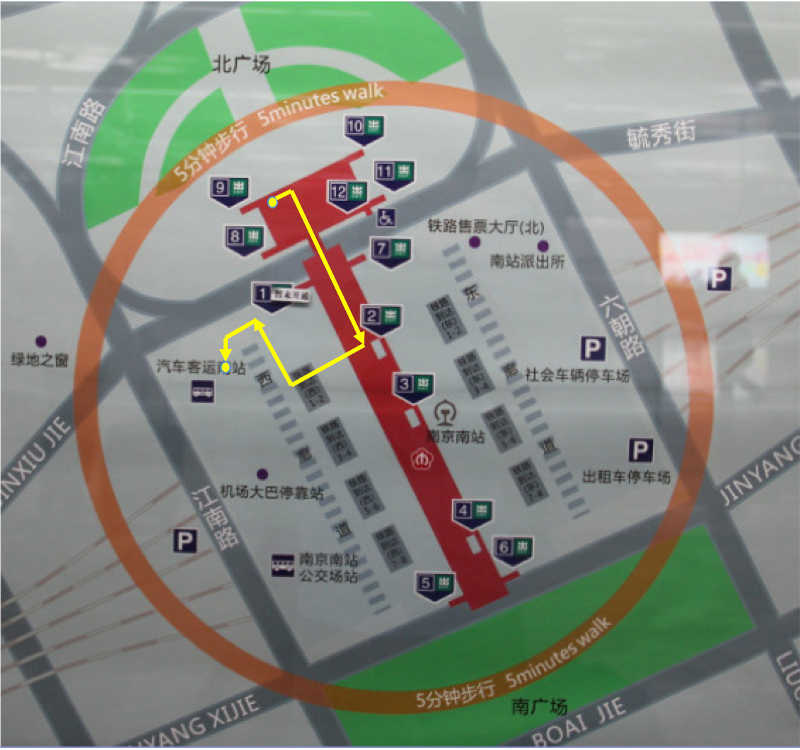
\includegraphics[scale=0.4]{ggg.jpg}
    	\caption{Map of Nanjing South Railway Station.\label{ggg}}
 \end{figure}

The following figures show details along the way.

When you get off the metro, you need to take an escalator to go one level up, and then go the direction of Metro Line 1 and Line 3 (Fig.~\ref{IMG_7166}) and the Taxi stop is somewhere down the way.

% (turn right, {\bf do not} turn left and exit) . ????!!! Can you be sure it is definitely turn right??? It may % depends on which escalator you are taking.

 \begin{figure}[!h]
	\begin{minipage}[t]{.5\textwidth}
     	\centering
        	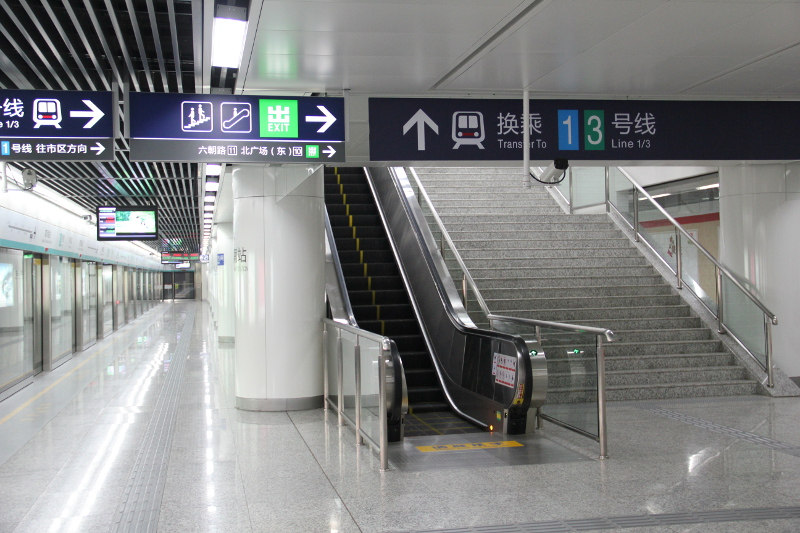
\includegraphics[scale=0.27]{IMG_7164.jpg}
	\end{minipage}%
     \begin{minipage}[t]{.5\textwidth}
         \centering
         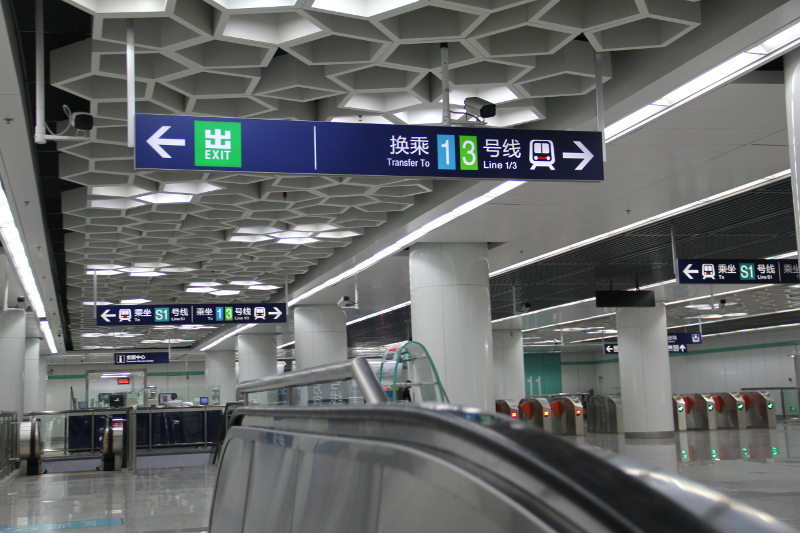
\includegraphics[scale=0.27]{IMG_7166.jpg}
    \end{minipage}%
    	\caption{The escalator you see when getting off Metro Line S1.\label{IMG_7166}}
 \end{figure}
 \begin{figure}[!h]
	\begin{minipage}[t]{.5\textwidth}
     	\centering
        	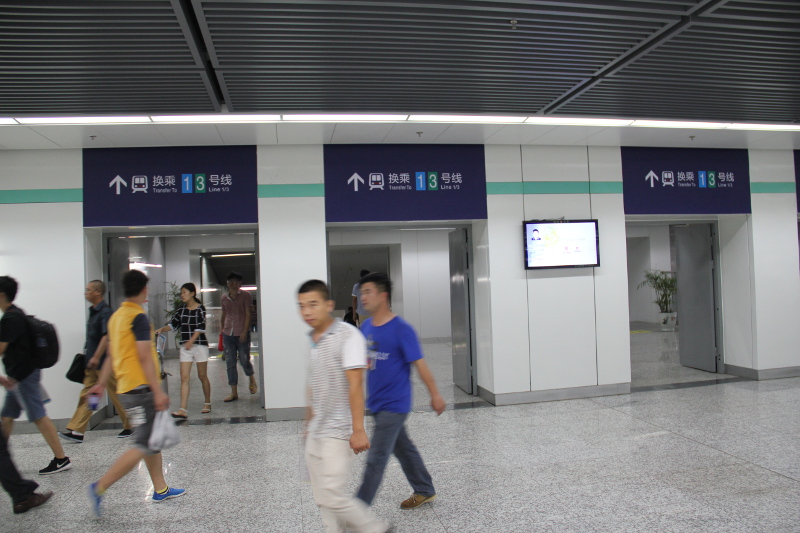
\includegraphics[scale=0.27]{IMG_7179.jpg}
		\caption{3 doors along the way.\label{IMG_7179}}
	\end{minipage}%
     \begin{minipage}[t]{.5\textwidth}
         \centering
       	 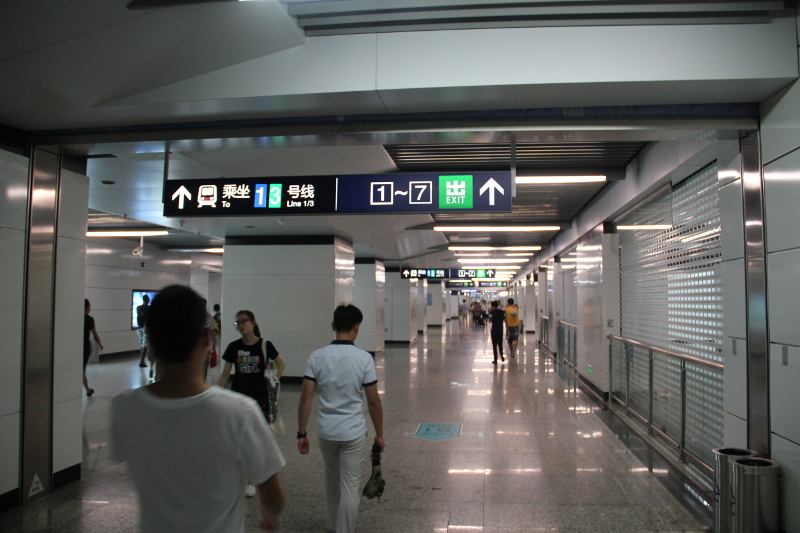
\includegraphics[scale=0.27]{IMG_7180.jpg}
		\caption{Continue and go towards exit 2B.\label{IMG_7180}}
    \end{minipage}%
 \end{figure}

 \begin{figure}[!h]
	\begin{minipage}[t]{.5\textwidth}
     	\centering
        	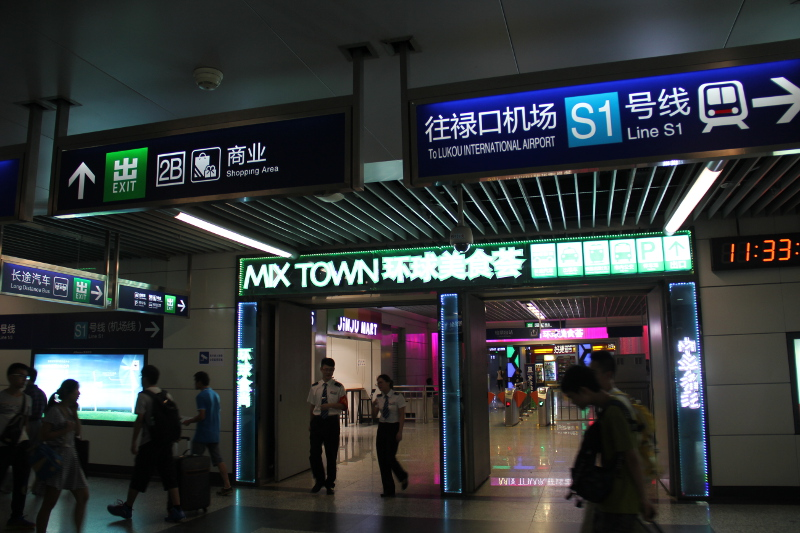
\includegraphics[scale=0.27]{IMG_7186.jpg}
	\end{minipage}%
     \begin{minipage}[t]{.5\textwidth}
         \centering
         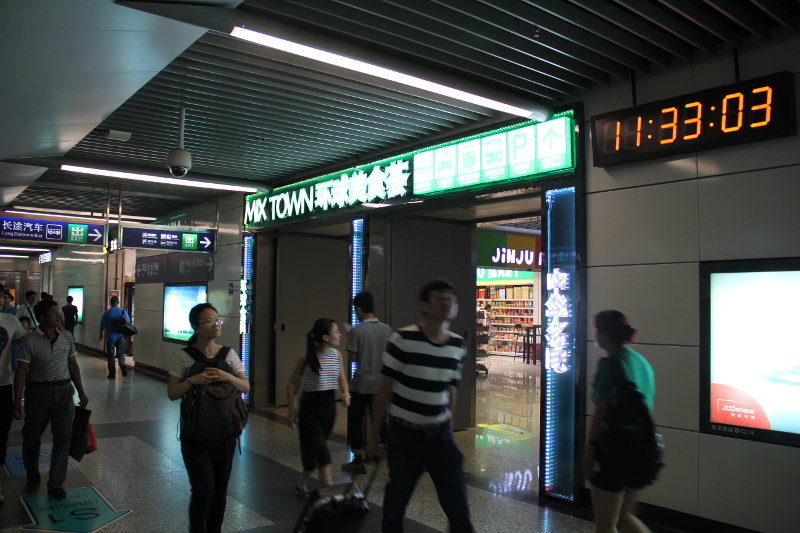
\includegraphics[scale=0.27]{IMG_7182.jpg}
    \end{minipage}%
    	\caption{Exit 2B.\label{IMG_7182}}
 \end{figure}
  \begin{figure}[!h]
	\begin{minipage}[t]{.5\textwidth}
     	\centering
        	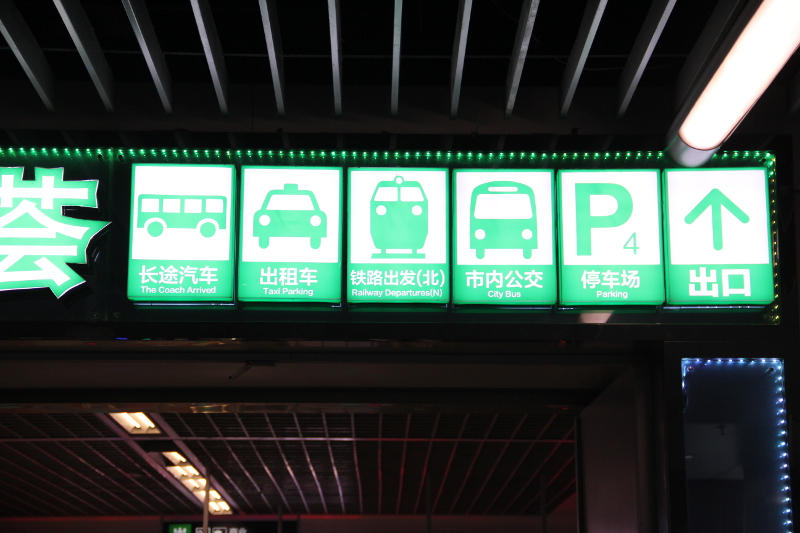
\includegraphics[scale=0.27]{IMG_7183.jpg}
    		\caption{Taxi sign at Exit 2B.\label{7183}}
	\end{minipage}%
     \begin{minipage}[t]{.5\textwidth}
         \centering
       	 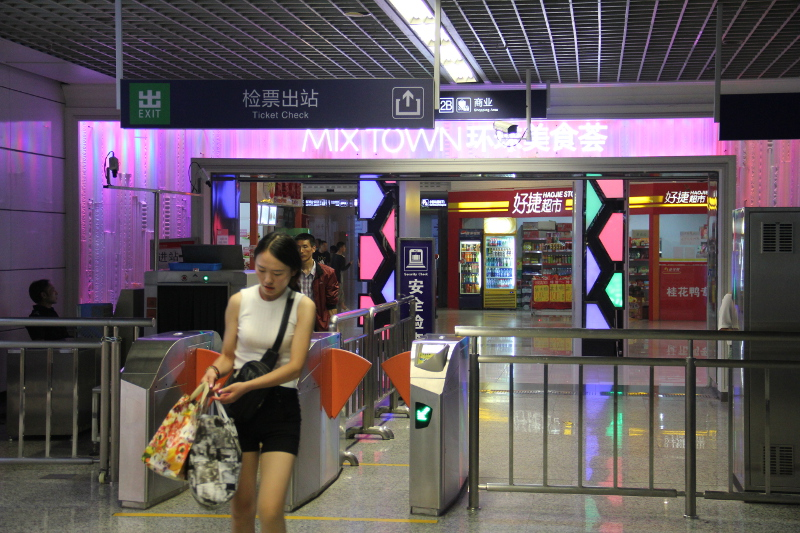
\includegraphics[scale=0.27]{IMG_7188.jpg}
		\caption{Exit through the ticket gate.\label{7188}}
    \end{minipage}%
 \end{figure}
 \begin{figure}[!h]
	\begin{minipage}[t]{.5\textwidth}
     	\centering
        	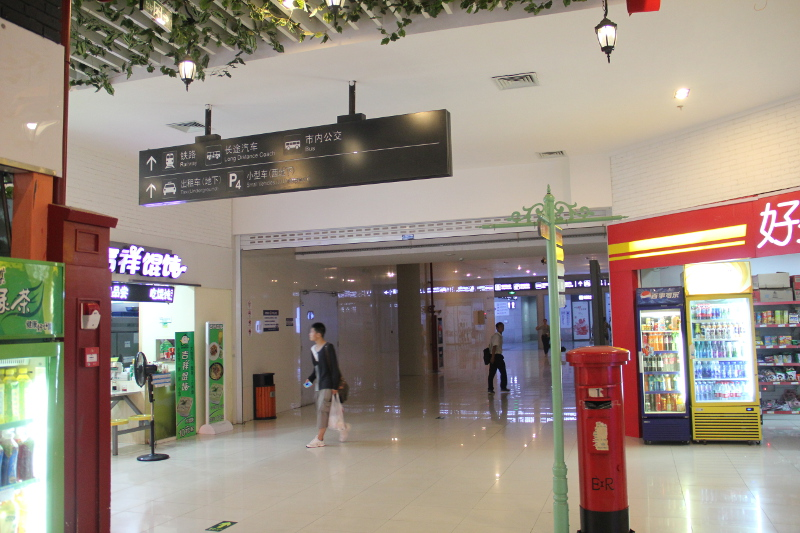
\includegraphics[scale=0.27]{IMG_7189.jpg}
	\end{minipage}%
     \begin{minipage}[t]{.5\textwidth}
         \centering
         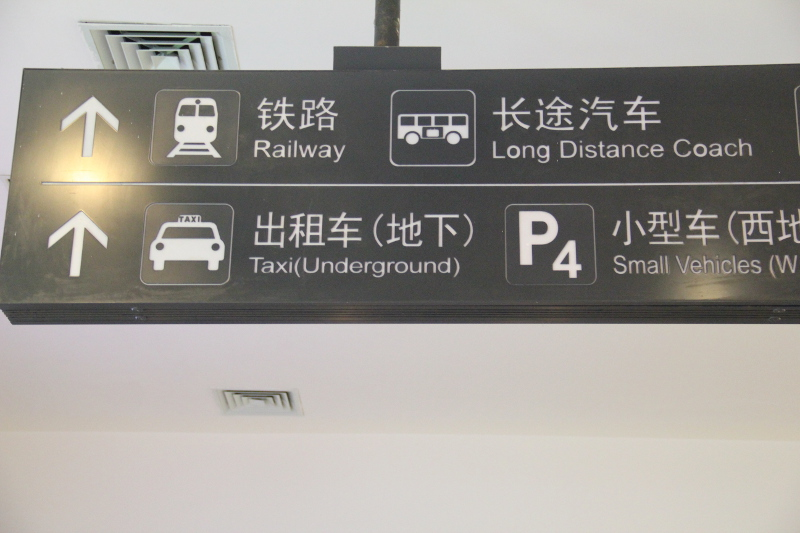
\includegraphics[scale=0.27]{IMG_7191.jpg}
    \end{minipage}%
    	\caption{Follow the direction to Taxi stop.\label{7191}}
 \end{figure}
 \begin{figure}[!h]
	\begin{minipage}[t]{.5\textwidth}
     	\centering
        	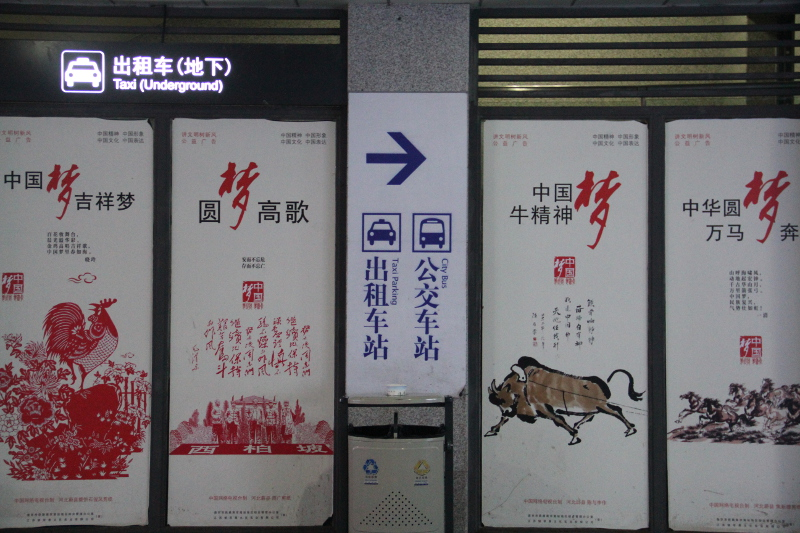
\includegraphics[scale=0.27]{IMG_7194.jpg} \\
		\caption{Turn right when you see these signs.\label{7194}}
	\end{minipage}%
     \begin{minipage}[t]{.5\textwidth}
         \centering
       	 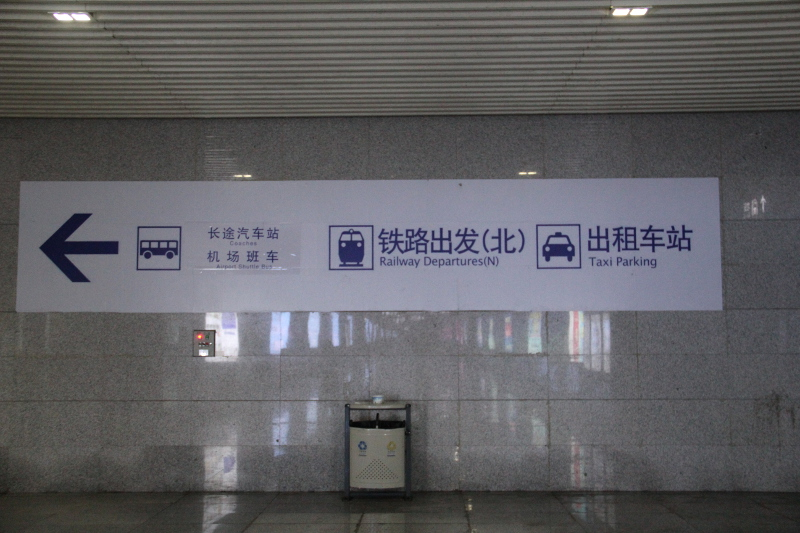
\includegraphics[scale=0.27]{IMG_7196.jpg} \\
	 	 \caption{Turn left at the end of the hall.\label{7194}}
    \end{minipage}%
 \end{figure}
  \begin{figure}[!h]
	\begin{minipage}[t]{.5\textwidth}
     	\centering
        	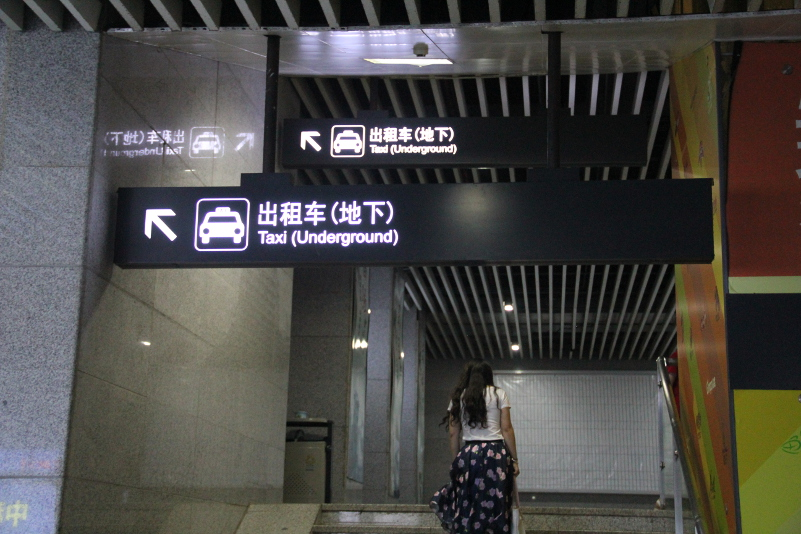
\includegraphics[scale=0.27]{IMG_7197.jpg}
		\caption{Follow the direction and go upstairs.\label{7197}}
	\end{minipage}%
     \begin{minipage}[t]{.5\textwidth}
         \centering
         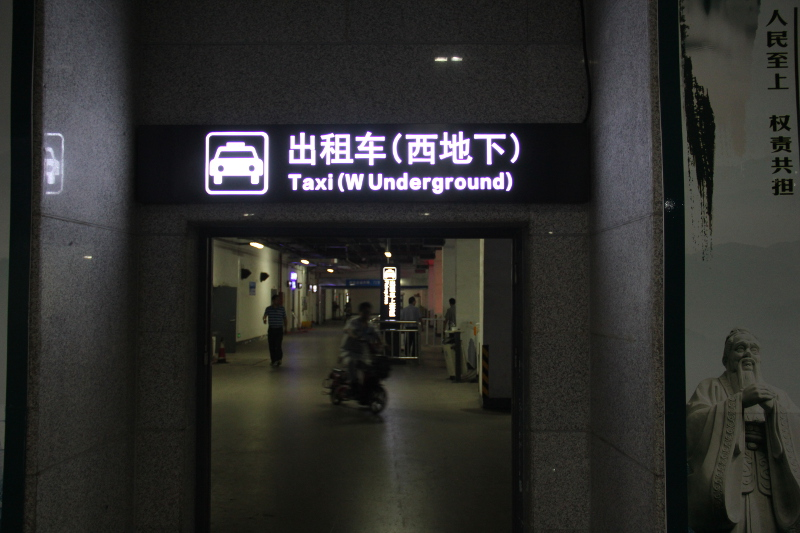
\includegraphics[scale=0.27]{IMG_7199.jpg}
         \caption{Go through this door.\label{7199}}
    \end{minipage}%    	
 \end{figure}
\begin{figure}[!h]
    \centering
    	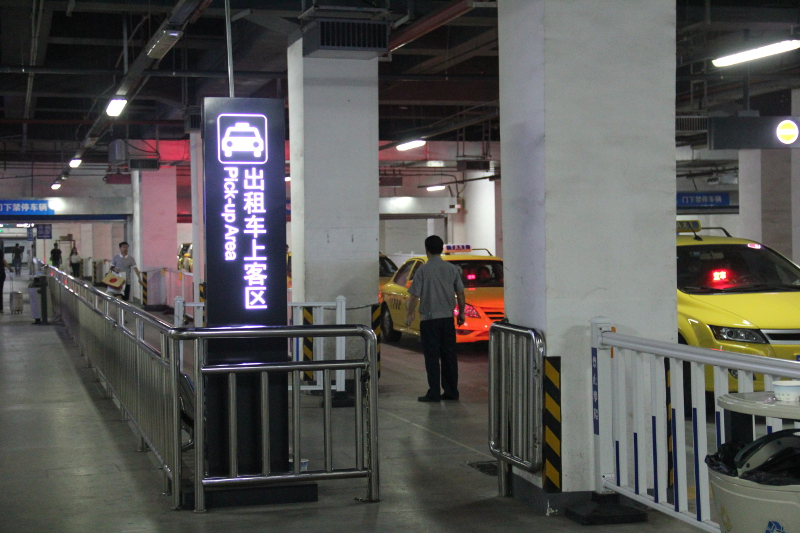
\includegraphics[scale=0.27]{IMG_7201.jpg}
    	\caption{Taxi stop is a few step ahead.\label{7201}}
 \end{figure}

  \clearpage

If you print out the following note and show it to the Taxi driver, he will understand where you want to go.

\begin{figure}[!h]
	 	\centering
	 司机师傅,请将我送往``{\bf 童卫路20号翰苑宾馆}'',其位置如地图中红色A点所示。\\
	 酒店电话:02584393962。谢谢!\\ \vspace{5mm}
     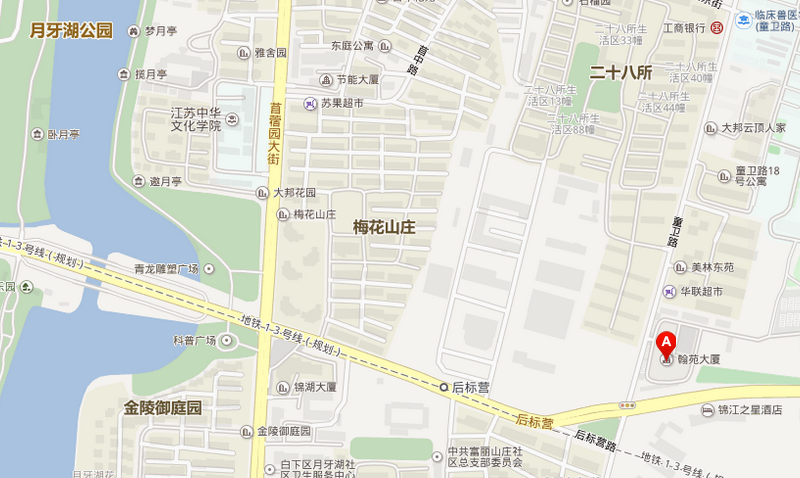
\includegraphics[scale=0.5]{badu.png}
\end{figure}

\section{Option 2}

If you take option 2, you can make a left turn when getting out the arrival gate (see Fig.~\ref{drawing}) and walk towards Exit 3 (Fig.~\ref{20150331_105629}).
The Texi spot is just outside Exit 3(Fig.~\ref{20150331_105836}).
\begin{figure}[!h]
	\begin{minipage}[t]{.5\textwidth}
     	\centering
   	 	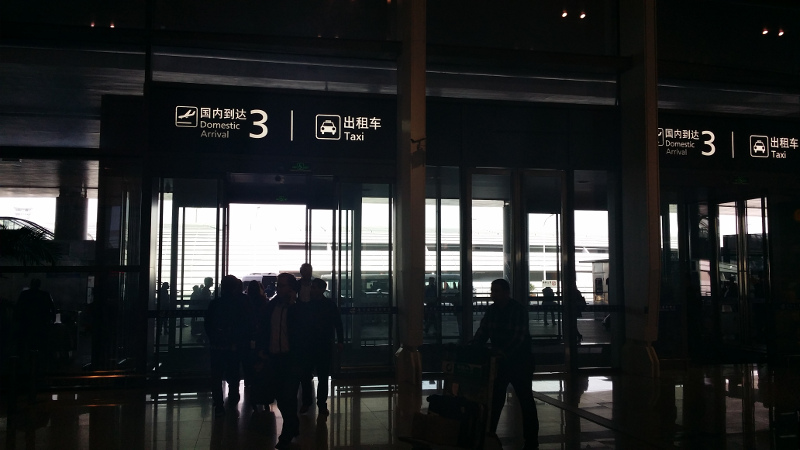
\includegraphics[scale=0.27]{20150331_105629.jpg}
    		\caption{Exit 3 for Taxi stop.\label{20150331_105629}}
	\end{minipage}%
     \begin{minipage}[t]{.5\textwidth}
         \centering
       	 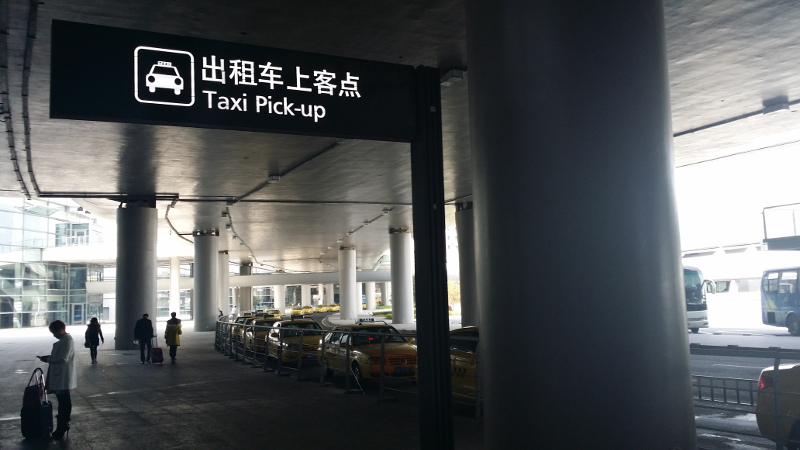
\includegraphics[scale=0.27]{20150331_105836.jpg} \\
	 	\caption{Taxi stop at airport.\label{20150331_105836}}
    \end{minipage}%
 \end{figure}

\section{Option 3}

Option 3 is {\bf not recommended}, the reason is that you need to get off the air shuttle bus in a middle stop (the second stop), but the driver does not speak English. However, if you are determined to go by air shuttle bus, walk through Exit 2 (see Fig.~\ref{20150331_103842}) and turn left to find the air shuttle ticket office (see Fig.~\ref{20150331_105706}).
\begin{figure}[!h]
	\begin{minipage}[t]{.5\textwidth}
     	\centering
   	 	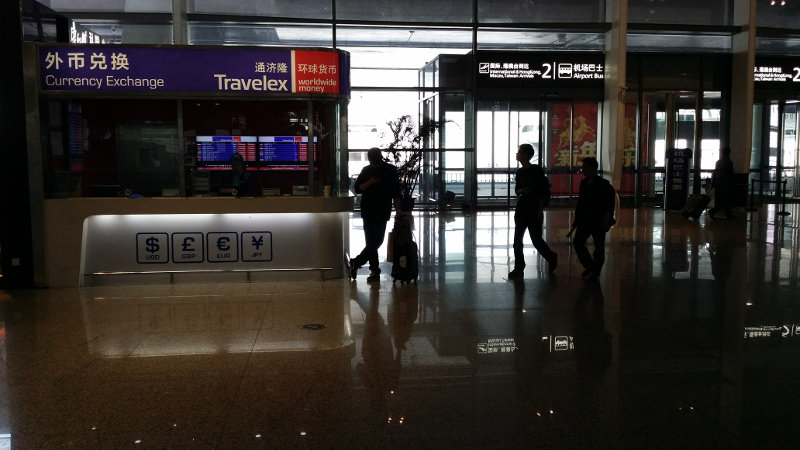
\includegraphics[scale=0.27]{20150331_103842.jpg}
    		\caption{Exit 2.\label{20150331_103842}}
	\end{minipage}%
     \begin{minipage}[t]{.5\textwidth}
         \centering
       	 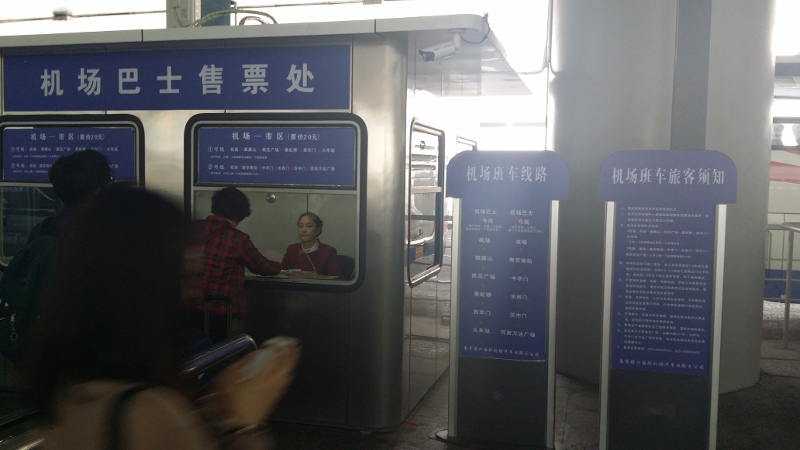
\includegraphics[scale=0.27]{20150331_105706.jpg} \\
	 	\caption{Ticket office of airport shuttles.\label{20150331_105706}}
    \end{minipage}%
 \end{figure}
 Buy a ticket for Bus Line 2 (20 RMB) and board at the scene shown in Fig.~\ref{20150331_104050}.
 \begin{figure}[!h]
	\begin{minipage}[t]{.5\textwidth}
     	\centering
   	 	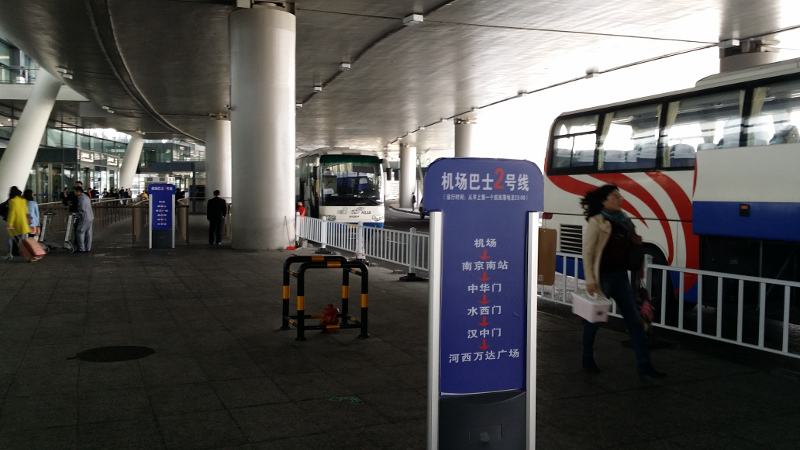
\includegraphics[scale=0.27]{20150331_104050.jpg}
	\end{minipage}%
     \begin{minipage}[t]{.5\textwidth}
         \centering
       	 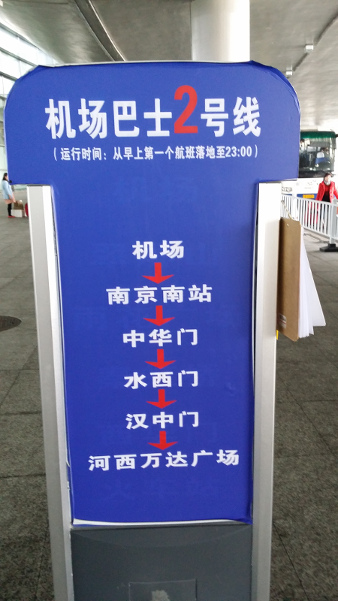
\includegraphics[scale=0.27]{20150331_104141.jpg} \\
    \end{minipage}%
    \caption{Wait at Bus Line 2.\label{20150331_104050}}
 \end{figure}
You need to get off the air shuttle bus at Nanjing South Railway Station (the second stop) and then
follow the directions towards the Taxi stop and show Taxi driver the following note, which tells where the Hanyuan hotel is.
\begin{center}
	 司机师傅,请将我送往``{\bf 童卫路20号翰苑宾馆}'',谢谢!
\end{center}

\end{document} 